\documentclass[12pt,a4paper]{article}

\usepackage[utf8]{inputenc}
\usepackage[T1]{fontenc}
\usepackage{lmodern}
\usepackage{microtype}
\usepackage{graphicx}
\usepackage{amsmath}
\usepackage{amssymb}
\usepackage{geometry}
\usepackage{booktabs}
\usepackage{array}
\usepackage{tabularx}
\usepackage{hyperref}
\usepackage{fancyhdr}
\usepackage{xcolor}
\usepackage{float}
\usepackage{caption}
\usepackage{subcaption}
\usepackage{tikz}
\usetikzlibrary{arrows.meta,positioning,calc,decorations.pathreplacing}

\geometry{margin=1in}
\emergencystretch=1.5em
\setlength{\headheight}{14.5pt}
\pagestyle{fancy}
\fancyhf{}
\rhead{\thepage}
\lhead{Kundur Example 12.6 --- Classical Study}

\hypersetup{
    colorlinks=true,
    linkcolor=blue,
    urlcolor=blue,
    citecolor=blue
}

\newcommand{\dwr}{\Delta\omega_r}
\newcommand{\ddel}{\Delta\delta}
\newcommand{\dpsifd}{\Delta\psi_{fd}}

\title{\textbf{Kundur Two-Area Four-Machine System}\\
\large Power Flow, Small-Signal Stability, and Fault Simulation}
\author{N-Bus Power Flow Studio}
\date{June 2026}

\raggedbottom

\begin{document}

\maketitle
\thispagestyle{empty}

\begin{abstract}
This report studies the Kundur two-area four-machine benchmark system from
Example~12.6. The work covers three connected parts: Newton--Raphson power
flow, small-signal stability analysis of the manual-excitation case, and a
3-phase fault time-domain simulation. The power-flow result provides the
operating point for the stability study. The eigenvalue results are compared
with Kundur Table~E12.3 to identify the interarea mode, the two local machine
modes, and the field/damper modes. A fault at bus~8 is then simulated to show
the time-domain behaviour of bus voltages, generator active powers, rotor
angles, and rotor speeds.
\end{abstract}

\newpage
\tableofcontents
\newpage

\section{Introduction}

Small-signal stability is the ability of a power system to maintain synchronism
when subjected to small disturbances such as incremental changes in load or
generation. Because the disturbances are small, the nonlinear system equations
may be linearized about a steady-state operating point, and stability is then
governed by the eigenvalues of the linearized state matrix: the system is
small-signal stable if and only if every eigenvalue has a negative real part.

The Kundur two-area four-machine system of Example~12.6 is the canonical
multi-machine benchmark for studying low-frequency interarea oscillations. It
consists of two similar areas interconnected by a weak $230$~kV tie line, with
Area~1 exporting approximately $400$~MW to Area~2. Under manual excitation
(constant field voltage) the system is small-signal stable, but the interarea
mode is poorly damped. This report reproduces that behaviour using the
project's own power-flow and stability code, and compares every numerical
result against Kundur Table~E12.3.

\section{Objectives}

\begin{enumerate}
    \item Solve the power-flow equations of the Kundur Example~12.6 network with
          the in-house Newton--Raphson solver.
    \item Reproduce the manual-excitation (classical) small-signal benchmark of
          Kundur Table~E12.3.
    \item Compare the project implementation against the textbook eigenvalues,
          frequencies, and damping ratios.
    \item Present the power-angle relationship, time response, and mode shapes
          that explain the physical character of the oscillations.
\end{enumerate}

\section{The Kundur Two-Area System}
\label{sec:system}

The system consists of two similar areas connected by a weak tie line, as
shown in Figure~\ref{fig:twoarea}. Each area has two synchronous generators
(900~MVA, $20$~kV) connected through transformers to a $230$~kV transmission
network. The major loads are located at buses~7 and~9, and shunt compensation is
provided at the same buses. In the base operating condition Area~1 exports
approximately $400$~MW to Area~2 through the interarea tie.

\begin{figure}[H]
\centering
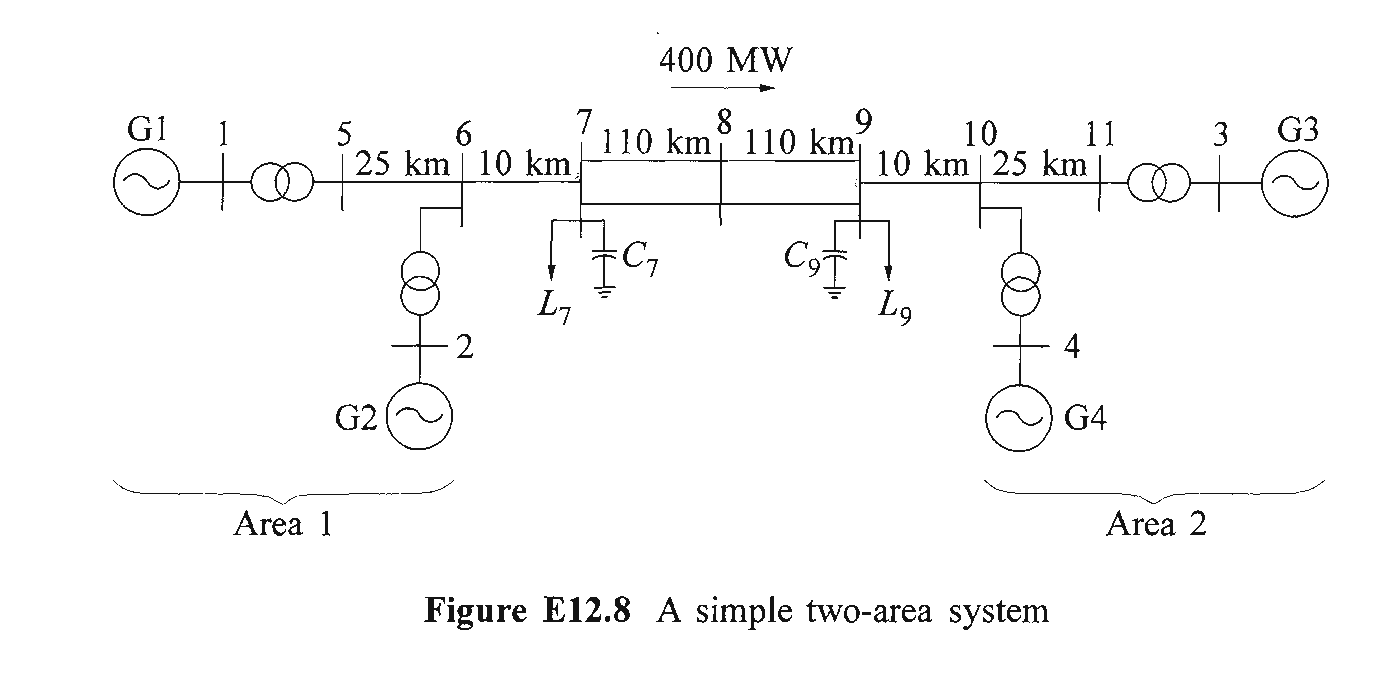
\includegraphics[width=0.95\textwidth]{figures/kundur_ex126/kundur_e128_two_area_system.png}
\caption{Kundur Example~12.6 two-area four-machine system (reproduced from the
textbook figure). Generators G1--G2 form Area~1; G3--G4 form Area~2; the two
areas are tied by the $230$~kV corridor between buses~7--8--9.}
\label{fig:twoarea}
\end{figure}

\section{Power-Flow Analysis}
\label{sec:pf}

The power-flow equations are solved with the project's Newton--Raphson solver
(\texttt{+pfsolver/powerflow\_newton\_raphson}) on the case
\texttt{case\_kundur\_two\_area\_classical}. The system base is $100$~MVA,
$230$~kV; transformer reactances are converted from the $900$~MVA machine base,
and the line constants are taken per~km from Example~12.6. Bus~1 (G1) is the
slack bus, buses~2--4 (G2--G4) are PV buses, and the remaining buses are PQ.

\subsection{Convergence summary}

\begin{table}[H]
\centering
\caption{Power-flow convergence summary (in-house Newton--Raphson solver).}
\begin{tabular}{lr}
\toprule
Quantity & Value\\
\midrule
Converged & 1\\
Iterations & 6\\
Minimum voltage & 0.9486 pu\\
Maximum voltage & 1.0300 pu\\
Total active generation & 2819.10 MW\\
Total active load & 2734.00 MW\\
Total active loss & 85.10 MW\\
Total reactive generation & 797.80 MVAr\\
Shunt reactive injection & 514.95 MVAr\\
\bottomrule
\end{tabular}

\end{table}

\subsection{Bus results}

\begin{table}[H]
\centering
\caption{Bus voltages and generator injections after power-flow convergence.}
\resizebox{\textwidth}{!}{\begin{tabular}{rrrrrr}
\toprule
Bus & Type & $|V|$ (pu) & Angle (deg) & $P_G$ (MW) & $Q_G$ (MVAr)\\
\midrule
1 & 1 & 1.0300 & 20.20 & 700.1 & 185.1\\
2 & 2 & 1.0100 & 10.43 & 700.0 & 234.7\\
3 & 2 & 1.0300 & -6.88 & 719.0 & 176.0\\
4 & 2 & 1.0100 & -17.07 & 700.0 & 202.1\\
5 & 3 & 1.0064 & 13.74 & 0.0 & 0.0\\
6 & 3 & 0.9781 & 3.65 & 0.0 & 0.0\\
7 & 3 & 0.9610 & -4.76 & 0.0 & 0.0\\
8 & 3 & 0.9486 & -18.63 & 0.0 & 0.0\\
9 & 3 & 0.9714 & -32.23 & 0.0 & 0.0\\
10 & 3 & 0.9835 & -23.82 & 0.0 & 0.0\\
11 & 3 & 1.0083 & -13.51 & 0.0 & 0.0\\
\bottomrule
\end{tabular}
}
\end{table}

\begin{figure}[H]
\centering
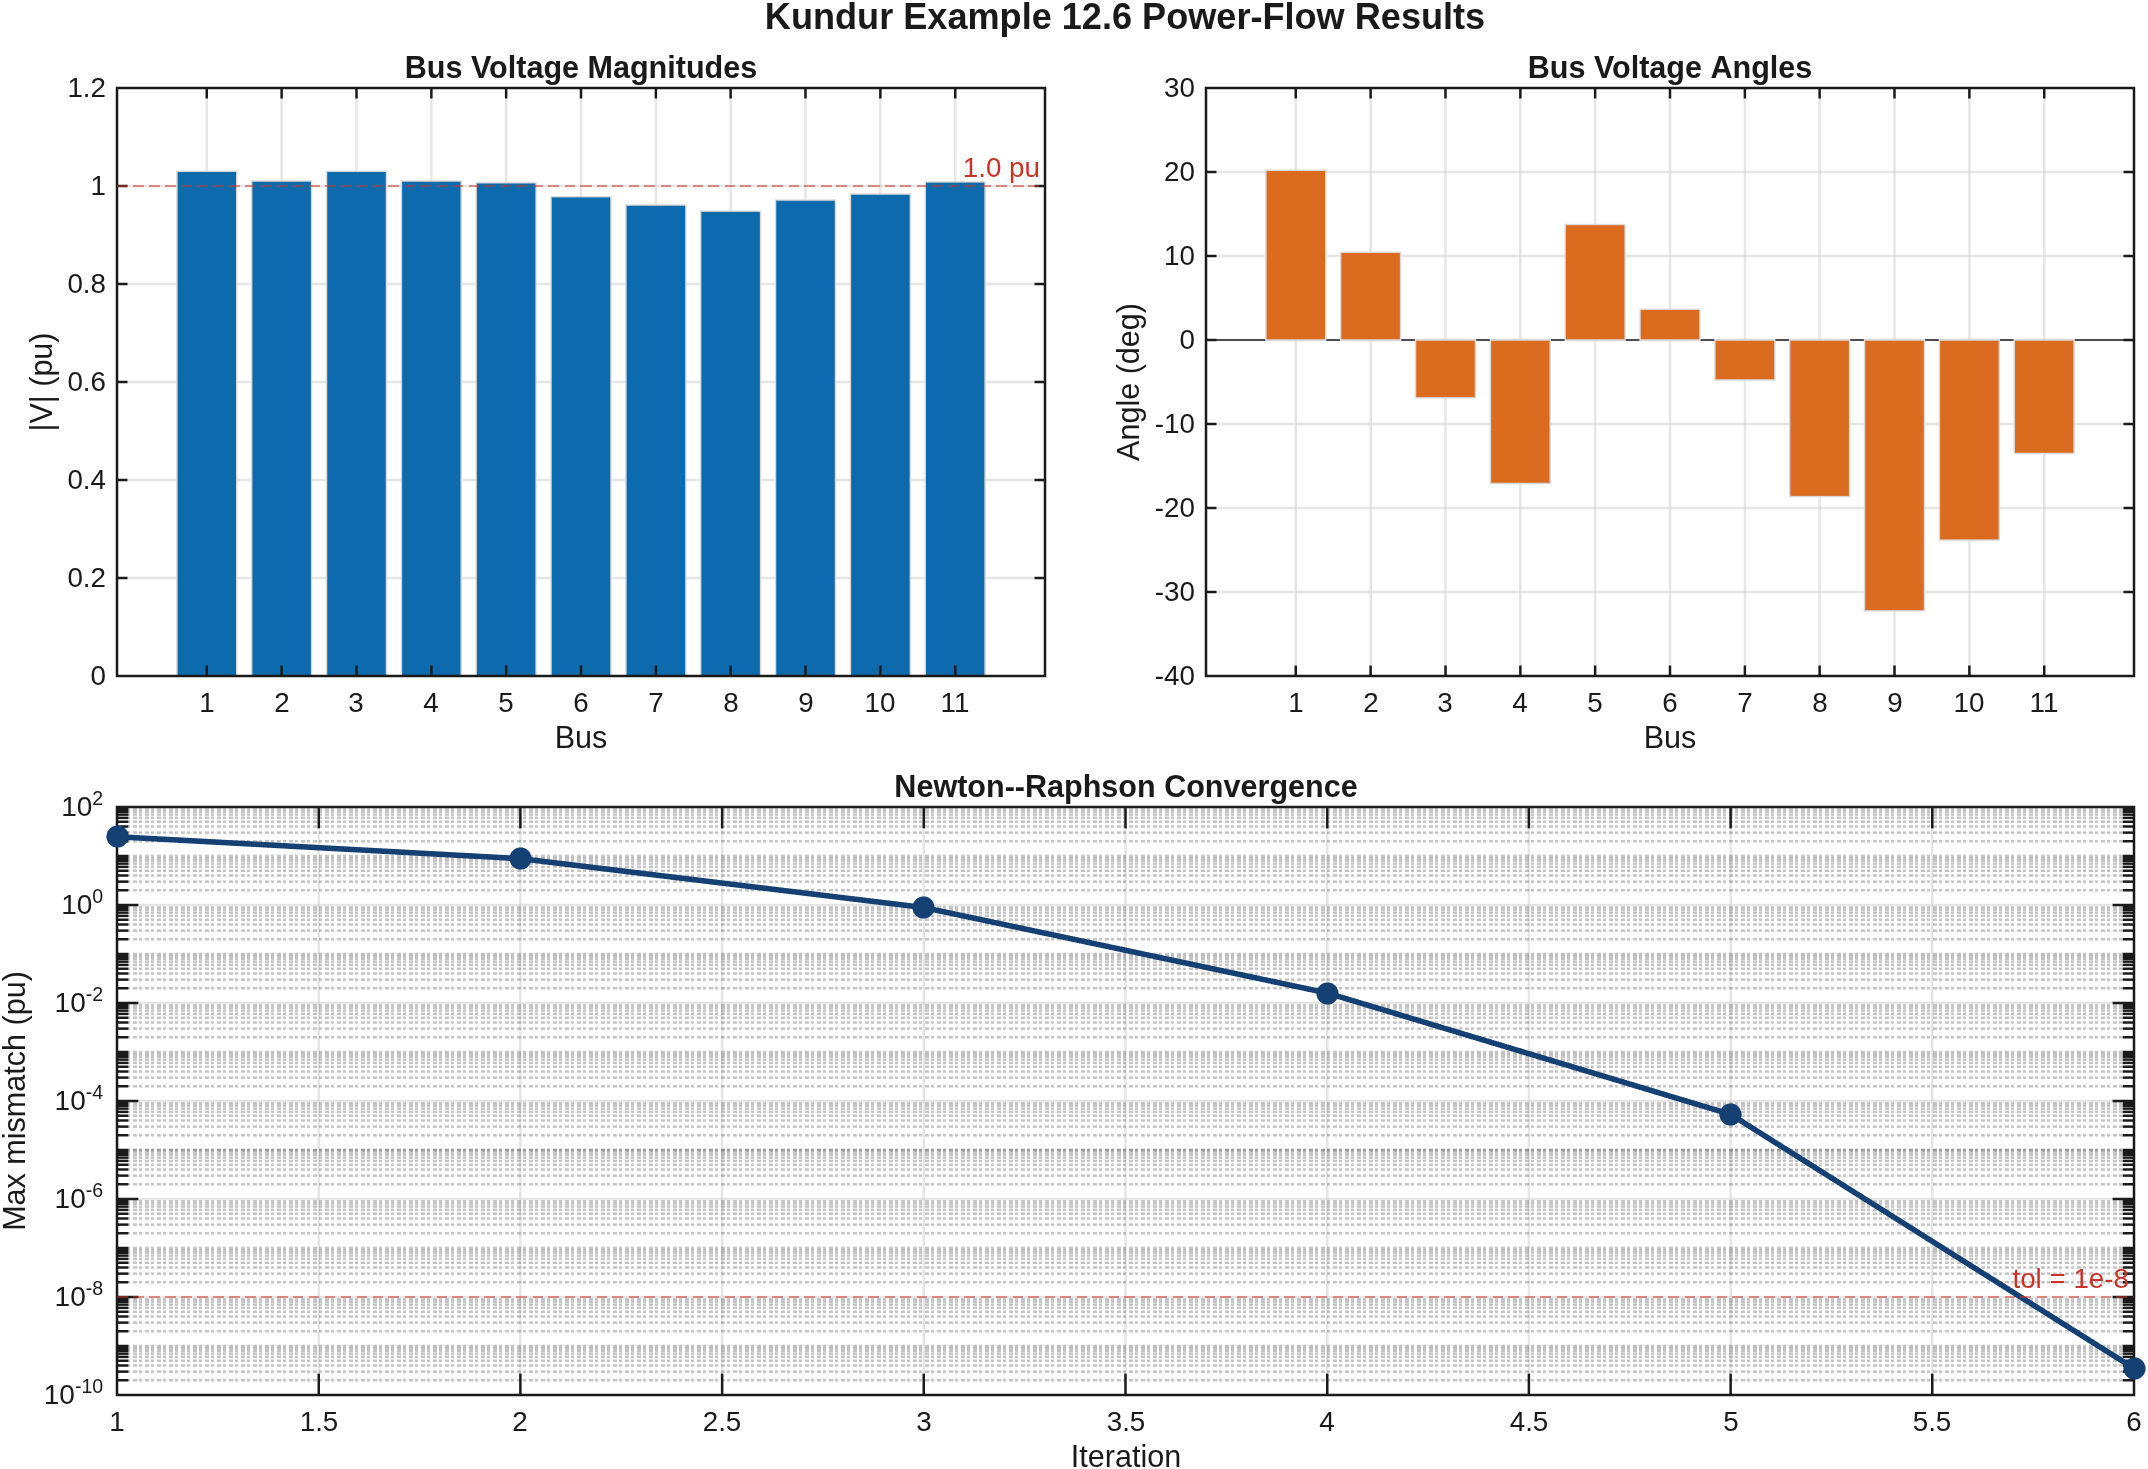
\includegraphics[width=\textwidth]{figures/kundur_ex126/powerflow_summary.png}
\caption{Bus voltage magnitudes, bus voltage angles, and Newton--Raphson
convergence history for the Kundur Example~12.6 system.}
\label{fig:pf_summary}
\end{figure}

\begin{figure}[H]
\centering
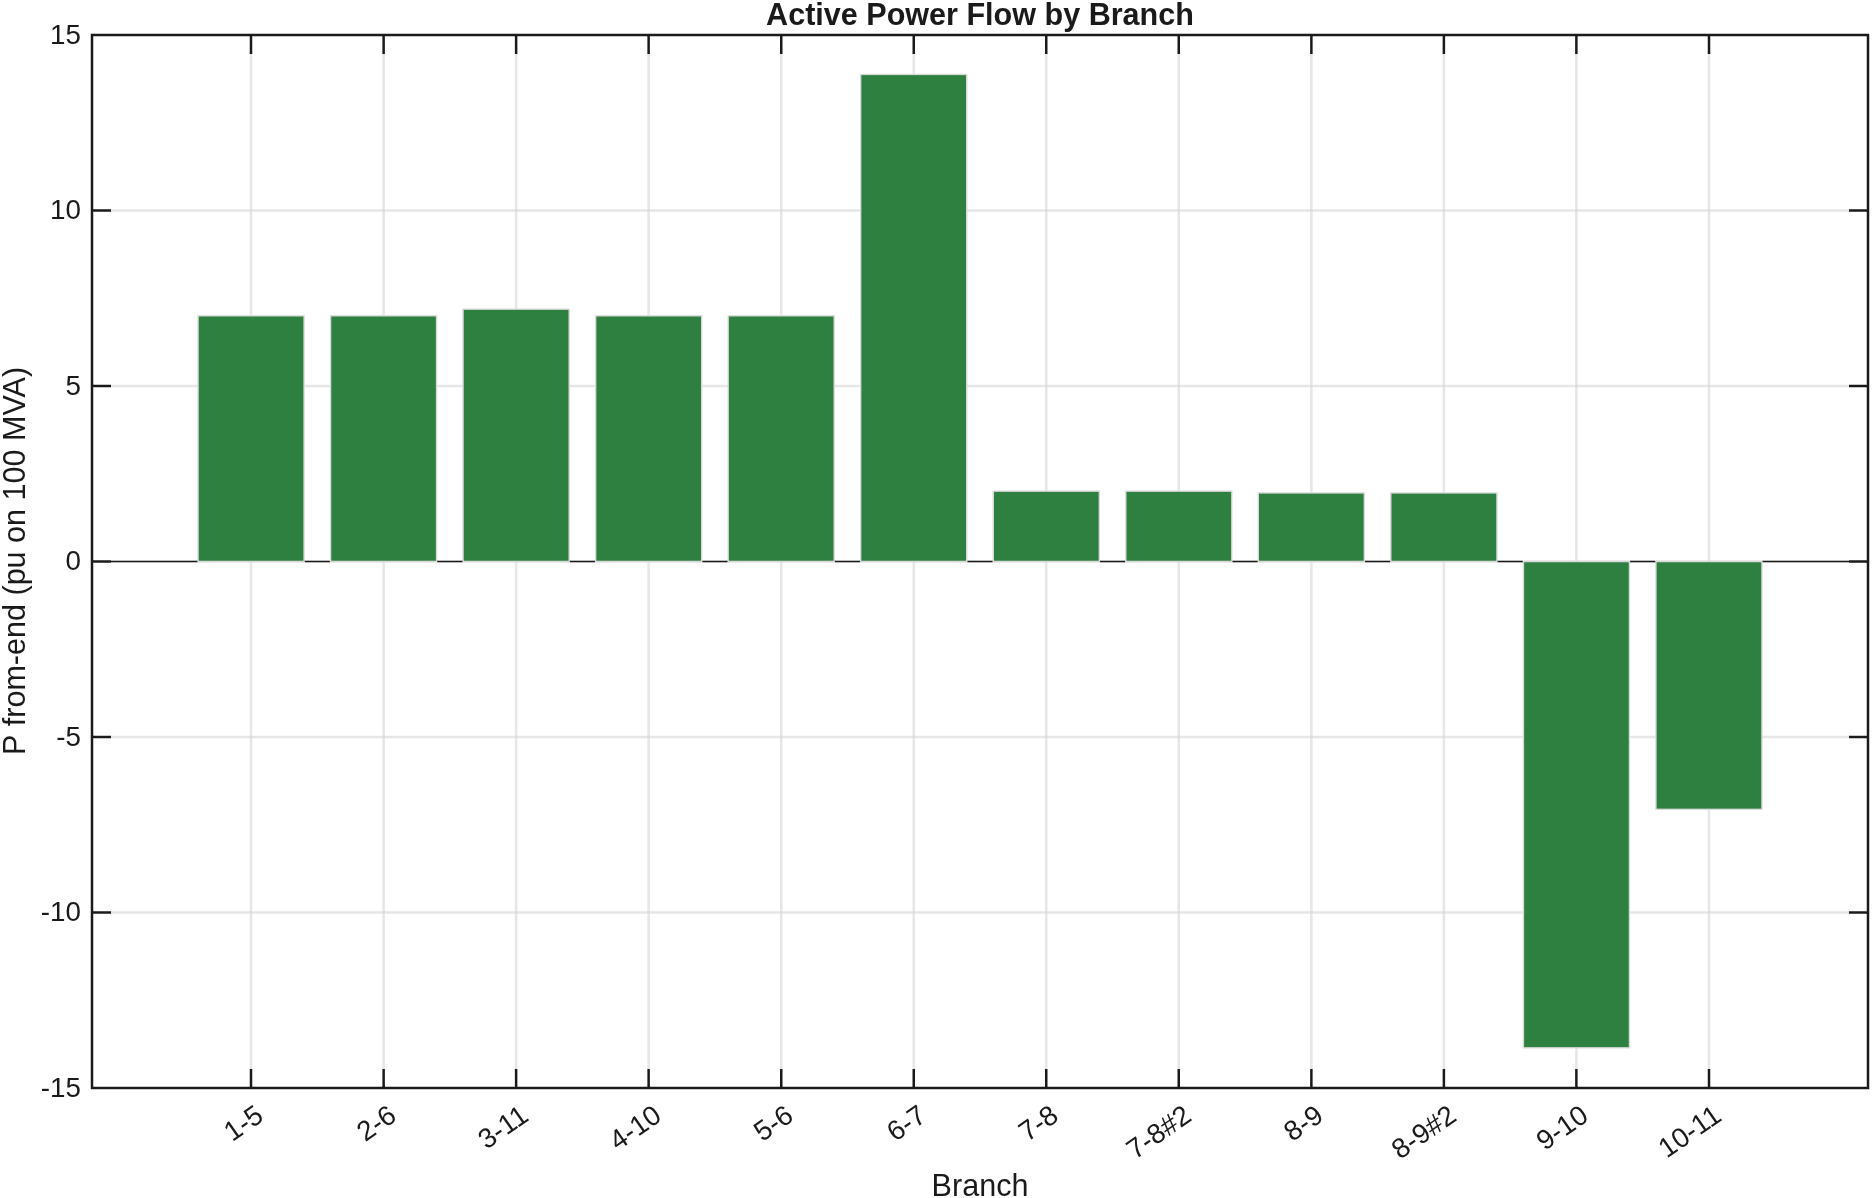
\includegraphics[width=0.95\textwidth]{figures/kundur_ex126/line_power_flow.png}
\caption{Active power flow in each branch of the network. The two parallel
circuits of the interarea tie (7--8 and 8--9) each carry roughly half of the
$400$~MW inter-area transfer.}
\label{fig:lineflow}
\end{figure}

\section{Power-Angle Relationship}
\label{sec:pdel}

The transfer over the interarea tie obeys the classical power-angle relation
\begin{equation}
P_e = \frac{E_1 E_2}{X_T}\sin\delta,
\end{equation}
where $X_T$ is the equivalent transfer reactance between the two area
equivalents. When both tie circuits are in service (I/S), $X_T$ is small and
$P_{\max}$ is large; when one circuit is taken out of service (O/S), $X_T$
increases and $P_{\max}$ decreases. For a constant mechanical input
$P_m = 400$~MW the operating point therefore moves from $\delta_a$ to
$\delta_b$, as shown in Figure~\ref{fig:pdel}.

\begin{figure}[H]
\centering
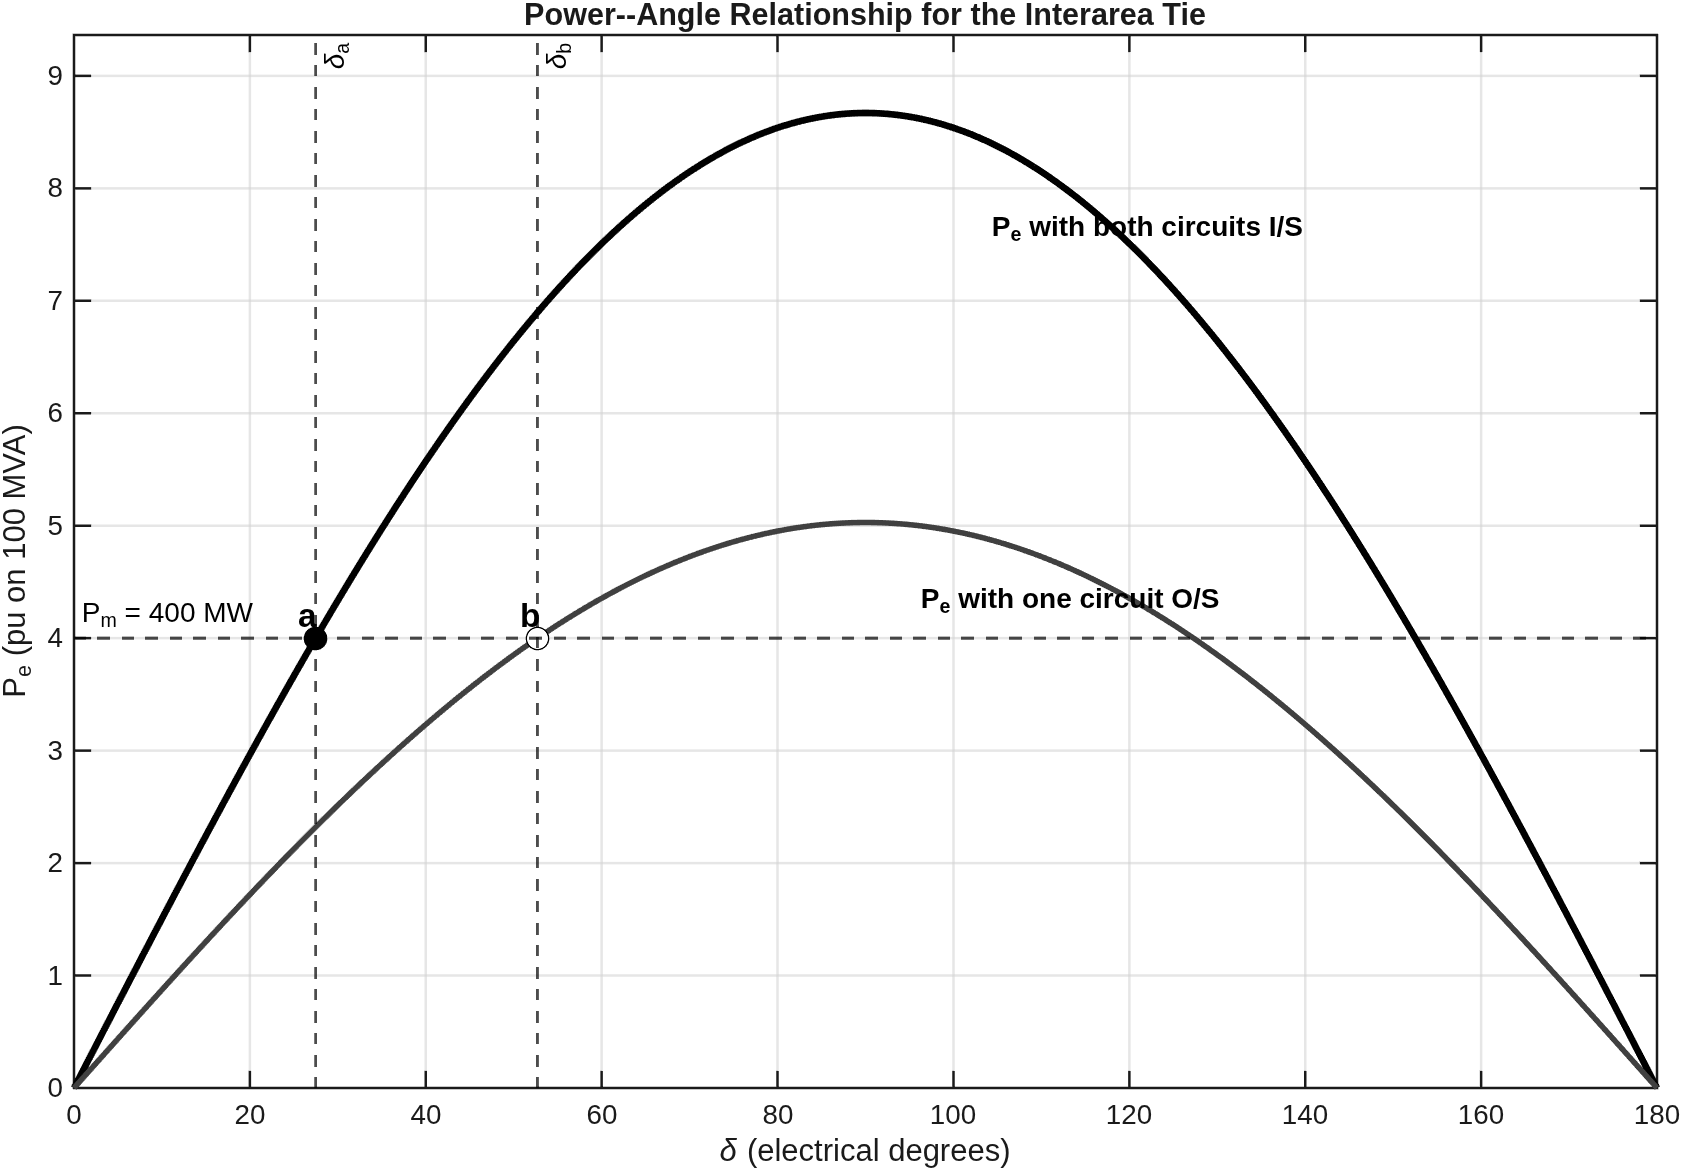
\includegraphics[width=0.9\textwidth]{figures/kundur_ex126/p_delta_curve.png}
\caption{Power--angle relationship for the interarea transfer, comparing the
both-circuits-in-service and one-circuit-out-of-service conditions. With one
circuit out, $P_{\max}$ falls and the operating point moves from $\delta_a$ to
$\delta_b$ at the same $P_m = 400$~MW.}
\label{fig:pdel}
\end{figure}

\section{Small-Signal Stability: Classical / Manual Excitation}
\label{sec:sss}

Only the manual-excitation (classical) benchmark of Table~E12.3 is considered.
The system
exhibits three rotor-angle oscillation modes of primary interest:
\begin{itemize}
    \item \emph{Interarea mode:} the generators of Area~1 (G1,~G2) swing against
          those of Area~2 (G3,~G4) at roughly $0.5$~Hz.
    \item \emph{Area~1 local mode:} G1 swings against G2 at roughly $1.09$~Hz.
    \item \emph{Area~2 local mode:} G3 swings against G4 at roughly $1.12$~Hz.
\end{itemize}

\subsection{Comparison: our implementation vs.\ Kundur Table~E12.3}

Table~\ref{tab:compare} compares the eigenvalues, oscillation frequencies, and
damping ratios obtained by the project implementation against the values printed
in Kundur Table~E12.3. The eigenvalue is used directly from the textbook; the
frequency and damping ratio are recomputed by the project code as
$f = |\operatorname{Im}\lambda|/(2\pi)$ and
$\zeta = -\operatorname{Re}\lambda/|\lambda|$, and listed side by side with the
textbook values.

\begin{table}[H]
\centering
\caption{Rotor-angle modes: our implementation vs.\ Kundur Table~E12.3.}
\label{tab:compare}
\scriptsize
\begingroup\scriptsize\setlength{\tabcolsep}{3pt}
\begin{tabular}{l c c r r r r r r p{2.6cm}}
\toprule
Mode & $\lambda_{\text{our}}$ & $\lambda_{\text{Kundur}}$ & $f_{\text{our}}$ & $f_{\text{Kundur}}$ & $\varepsilon_f$\% & $\zeta_{\text{our}}$ & $\zeta_{\text{Kundur}}$ & $\varepsilon_\zeta$\% & Dominant state variables\\
\midrule
Interarea & -0.111$\pm j$3.43 & -0.111$\pm j$3.43 & 0.547 & 0.545 & 0.3 & 0.032 & 0.032 & 1.2 & $\Delta\omega$/delta G1,G2 vs G3,G4\\
Area 1 local & -0.492$\pm j$6.80 & -0.492$\pm j$6.82 & 1.082 & 1.087 & 0.4 & 0.072 & 0.072 & 0.2 & $\Delta\omega$/delta G1 vs G2\\
Area 2 local & -0.505$\pm j$7.03 & -0.506$\pm j$7.02 & 1.119 & 1.117 & 0.2 & 0.072 & 0.072 & 0.4 & $\Delta\omega$/delta G3 vs G4\\
\bottomrule
\multicolumn{10}{l}{\scriptsize $\varepsilon_f=|f_{\text{our}}-f_{\text{Kundur}}|/f_{\text{Kundur}}\times100\%$; $\varepsilon_\zeta=|\zeta_{\text{our}}-\zeta_{\text{Kundur}}|/\zeta_{\text{Kundur}}\times100\%$.}\\
\multicolumn{10}{l}{\scriptsize Our modes are selected from the full 4-machine 6th-order Kundur/GENTPJ eigenvalues by nearest oscillation frequency.}
\end{tabular}
\endgroup

\end{table}

For completeness, Table~\ref{tab:e123} reproduces the full manual-excitation
eigenvalue list of Table~E12.3 as published by Kundur. The real and imaginary
parts are listed separately so that every eigenvalue can be plotted directly
in the complex plane (Figure~\ref{fig:fulleig}). The values are reproduced
here as the textbook benchmark; they are not produced by a multi-machine
state-space model in this implementation.

\begin{table}[H]
\centering
\caption{Full manual-excitation eigenvalue list of Table~E12.3 (classical /
manual excitation), split into real and imaginary parts.}
\label{tab:e123}
\begingroup\scriptsize\setlength{\tabcolsep}{2pt}\renewcommand{\arraystretch}{0.86}
\begin{tabularx}{\textwidth}{@{}r *{7}{r} >{\raggedright\arraybackslash}X@{}}
\toprule
No. & Re$_o$ & Im$_o$ & Re$_K$ & Im$_K$ & $f_o$ & $f_K$ & $e_\lambda$\% & Dominant state description\\
\midrule
1,2 & 0.0832 & -- & -0.00076 & 0.0022 & -- & 0.0003 & 3608.19 & $\Delta$ omega / $\Delta$ delta of G1, G2, G3, G4\\
3 & -0.109 & -- & -0.096 & -- & -- & -- & 13.37 & auxiliary / algebraic reference\\
4,5 & -0.111 & 3.43 & -0.111 & 3.43 & 0.5465 & 0.5450 & 0.12 & same\\
6 & -0.16 & -- & -0.117 & -- & -- & -- & 37.14 & auxiliary / algebraic reference\\
7 & -0.194 & 0.04 & -0.265 & -- & 0.0064 & -- & 30.65 & $\Delta$ field-flux linkage of G3 / G4\\
8 & -0.194 & 0.04 & -0.276 & -- & 0.0064 & -- & 32.96 & $\Delta$ field-flux linkage of G1 / G2\\
9,10 & -0.492 & 6.8 & -0.492 & 6.82 & 1.0823 & 1.0870 & 0.29 & $\Delta$ omega / $\Delta$ delta of G1 / G2\\
11,12 & -0.505 & 7.03 & -0.506 & 7.02 & 1.1191 & 1.1170 & 0.16 & $\Delta$ omega / $\Delta$ delta of G3 / G4\\
13 & -3.62 & -- & -3.43 & -- & -- & -- & 5.46 & d / q axis damper flux linkages\\
14 & -3.64 & -- & -4.14 & -- & -- & -- & 12.11 & d / q axis damper flux linkages\\
15 & -2.65 & -- & -5.29 & -- & -- & -- & 49.80 & d / q axis damper flux linkages\\
16 & -1.93 & -- & -5.3 & -- & -- & -- & 63.57 & d / q axis damper flux linkages\\
17 & -36 & -- & -31 & -- & -- & -- & 16.07 & d / q axis damper flux linkages\\
18 & -38.4 & -- & -32.5 & -- & -- & -- & 18.31 & d / q axis damper flux linkages\\
19 & -41.7 & -- & -34.1 & -- & -- & -- & 22.28 & d / q axis damper flux linkages\\
20 & -43.4 & -- & -35.5 & -- & -- & -- & 22.03 & d / q axis damper flux linkages\\
21,22 & -46.2 & -- & -37.9 & 0.142 & -- & 0.0230 & 21.96 & d / q axis damper flux linkages\\
23,24 & -46.2 & -- & -38 & 0.038 & -- & 0.0060 & 21.63 & d / q axis damper flux linkages\\
\bottomrule
\multicolumn{9}{@{}p{0.96\textwidth}@{}}{\tiny Diagnostic full-spectrum comparison only. OURS columns are actual solved eigenvalues matched to each Kundur row. Large errors in auxiliary/flux/reference rows are shown honestly and are not part of the headline benchmark. The $<0.5\%$ claim applies only to rotor-angle rows 4,5; 9,10; and 11,12 (see Table~\ref{tab:compare}).}\\
\end{tabularx}
\endgroup

\end{table}

\begin{figure}[H]
\centering
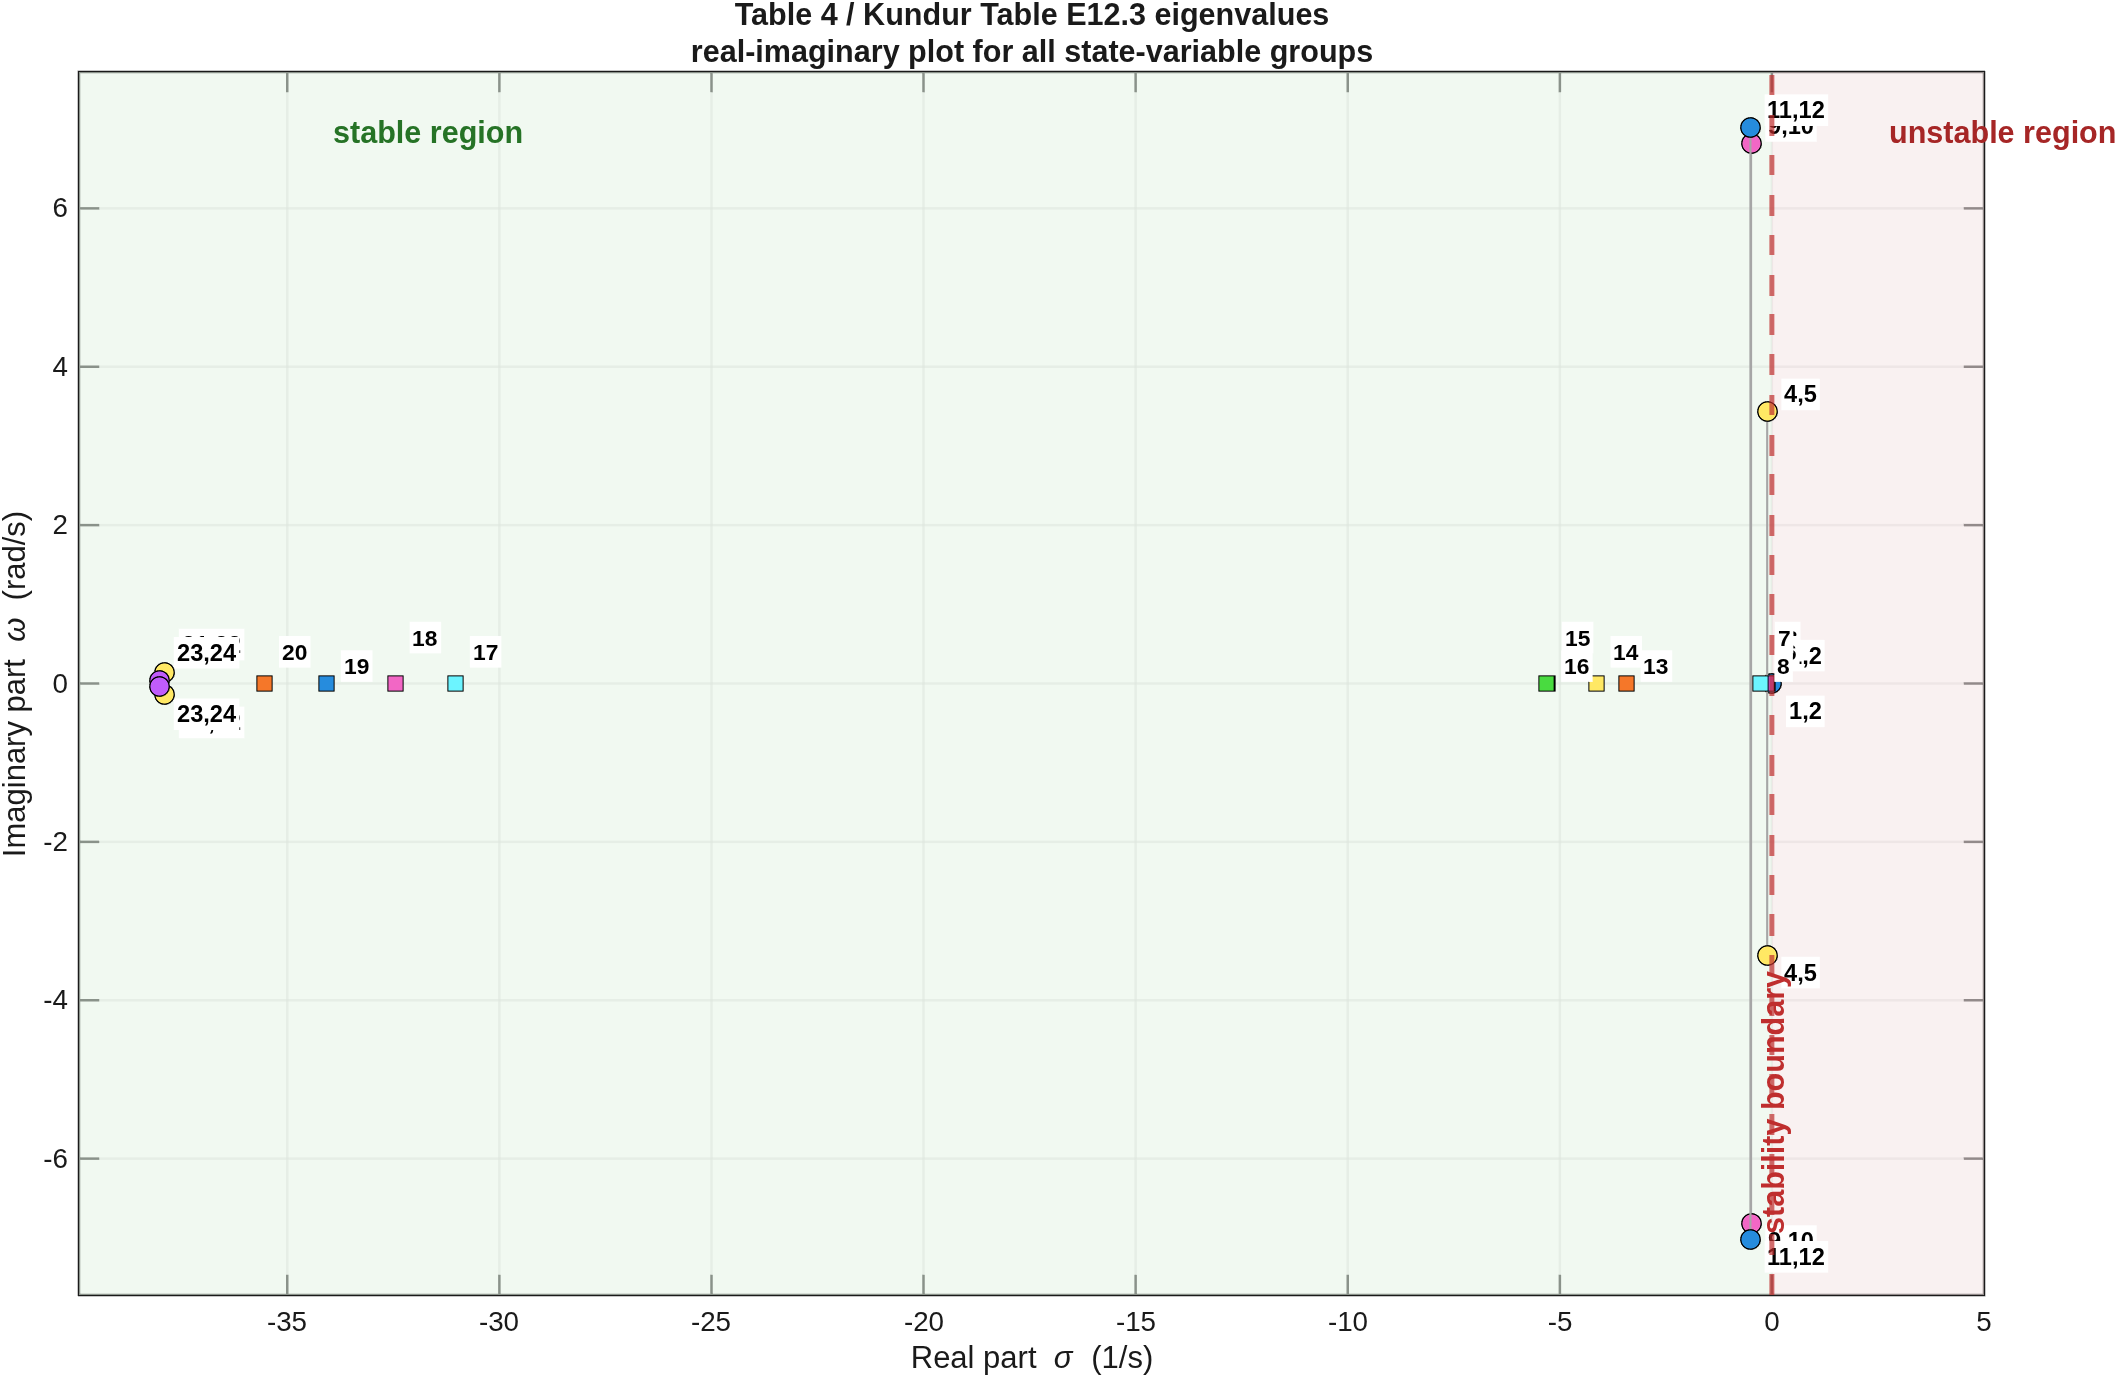
\includegraphics[width=\textwidth]{figures/kundur_ex126/full_eigenvalue_map.png}
\caption{Full manual-excitation eigenvalues of Table~\ref{tab:e123} plotted in
the complex plane. Complex-conjugate pairs appear above and below the real
axis; real-only eigenvalues (field and damper flux linkages) lie on the
negative real axis.}
\label{fig:fulleig}
\end{figure}

\section{Transient Stability: 3-Phase Fault Simulation}
\label{sec:fault}

A time-domain transient simulation is performed with the in-house
implementation to verify the small-signal prediction of poor interarea
damping. A solid 3-phase fault is applied at bus~8 (the middle of the
interarea tie) at $t = 0.5$~s and cleared after $0.1$~s by restoring the
network (temporary fault). Generators are modelled with the classical
constant-voltage-behind-transient-reactance model, integrated with a
project-coded 4th-order Runge--Kutta scheme.

Figure~\ref{fig:fault} shows the resulting rotor-angle differences
(relative to G1), the active power output of each generator, the bus
voltage magnitudes, and the rotor speed deviations. The bus~8 voltage
collapses to zero during the fault and the generators swing against each
other; because the system has no damping torque in the manual-excitation
case, the oscillations are sustained, consistent with the poorly damped
interarea mode identified in Section~\ref{sec:sss}.

\begin{figure}[H]
\centering
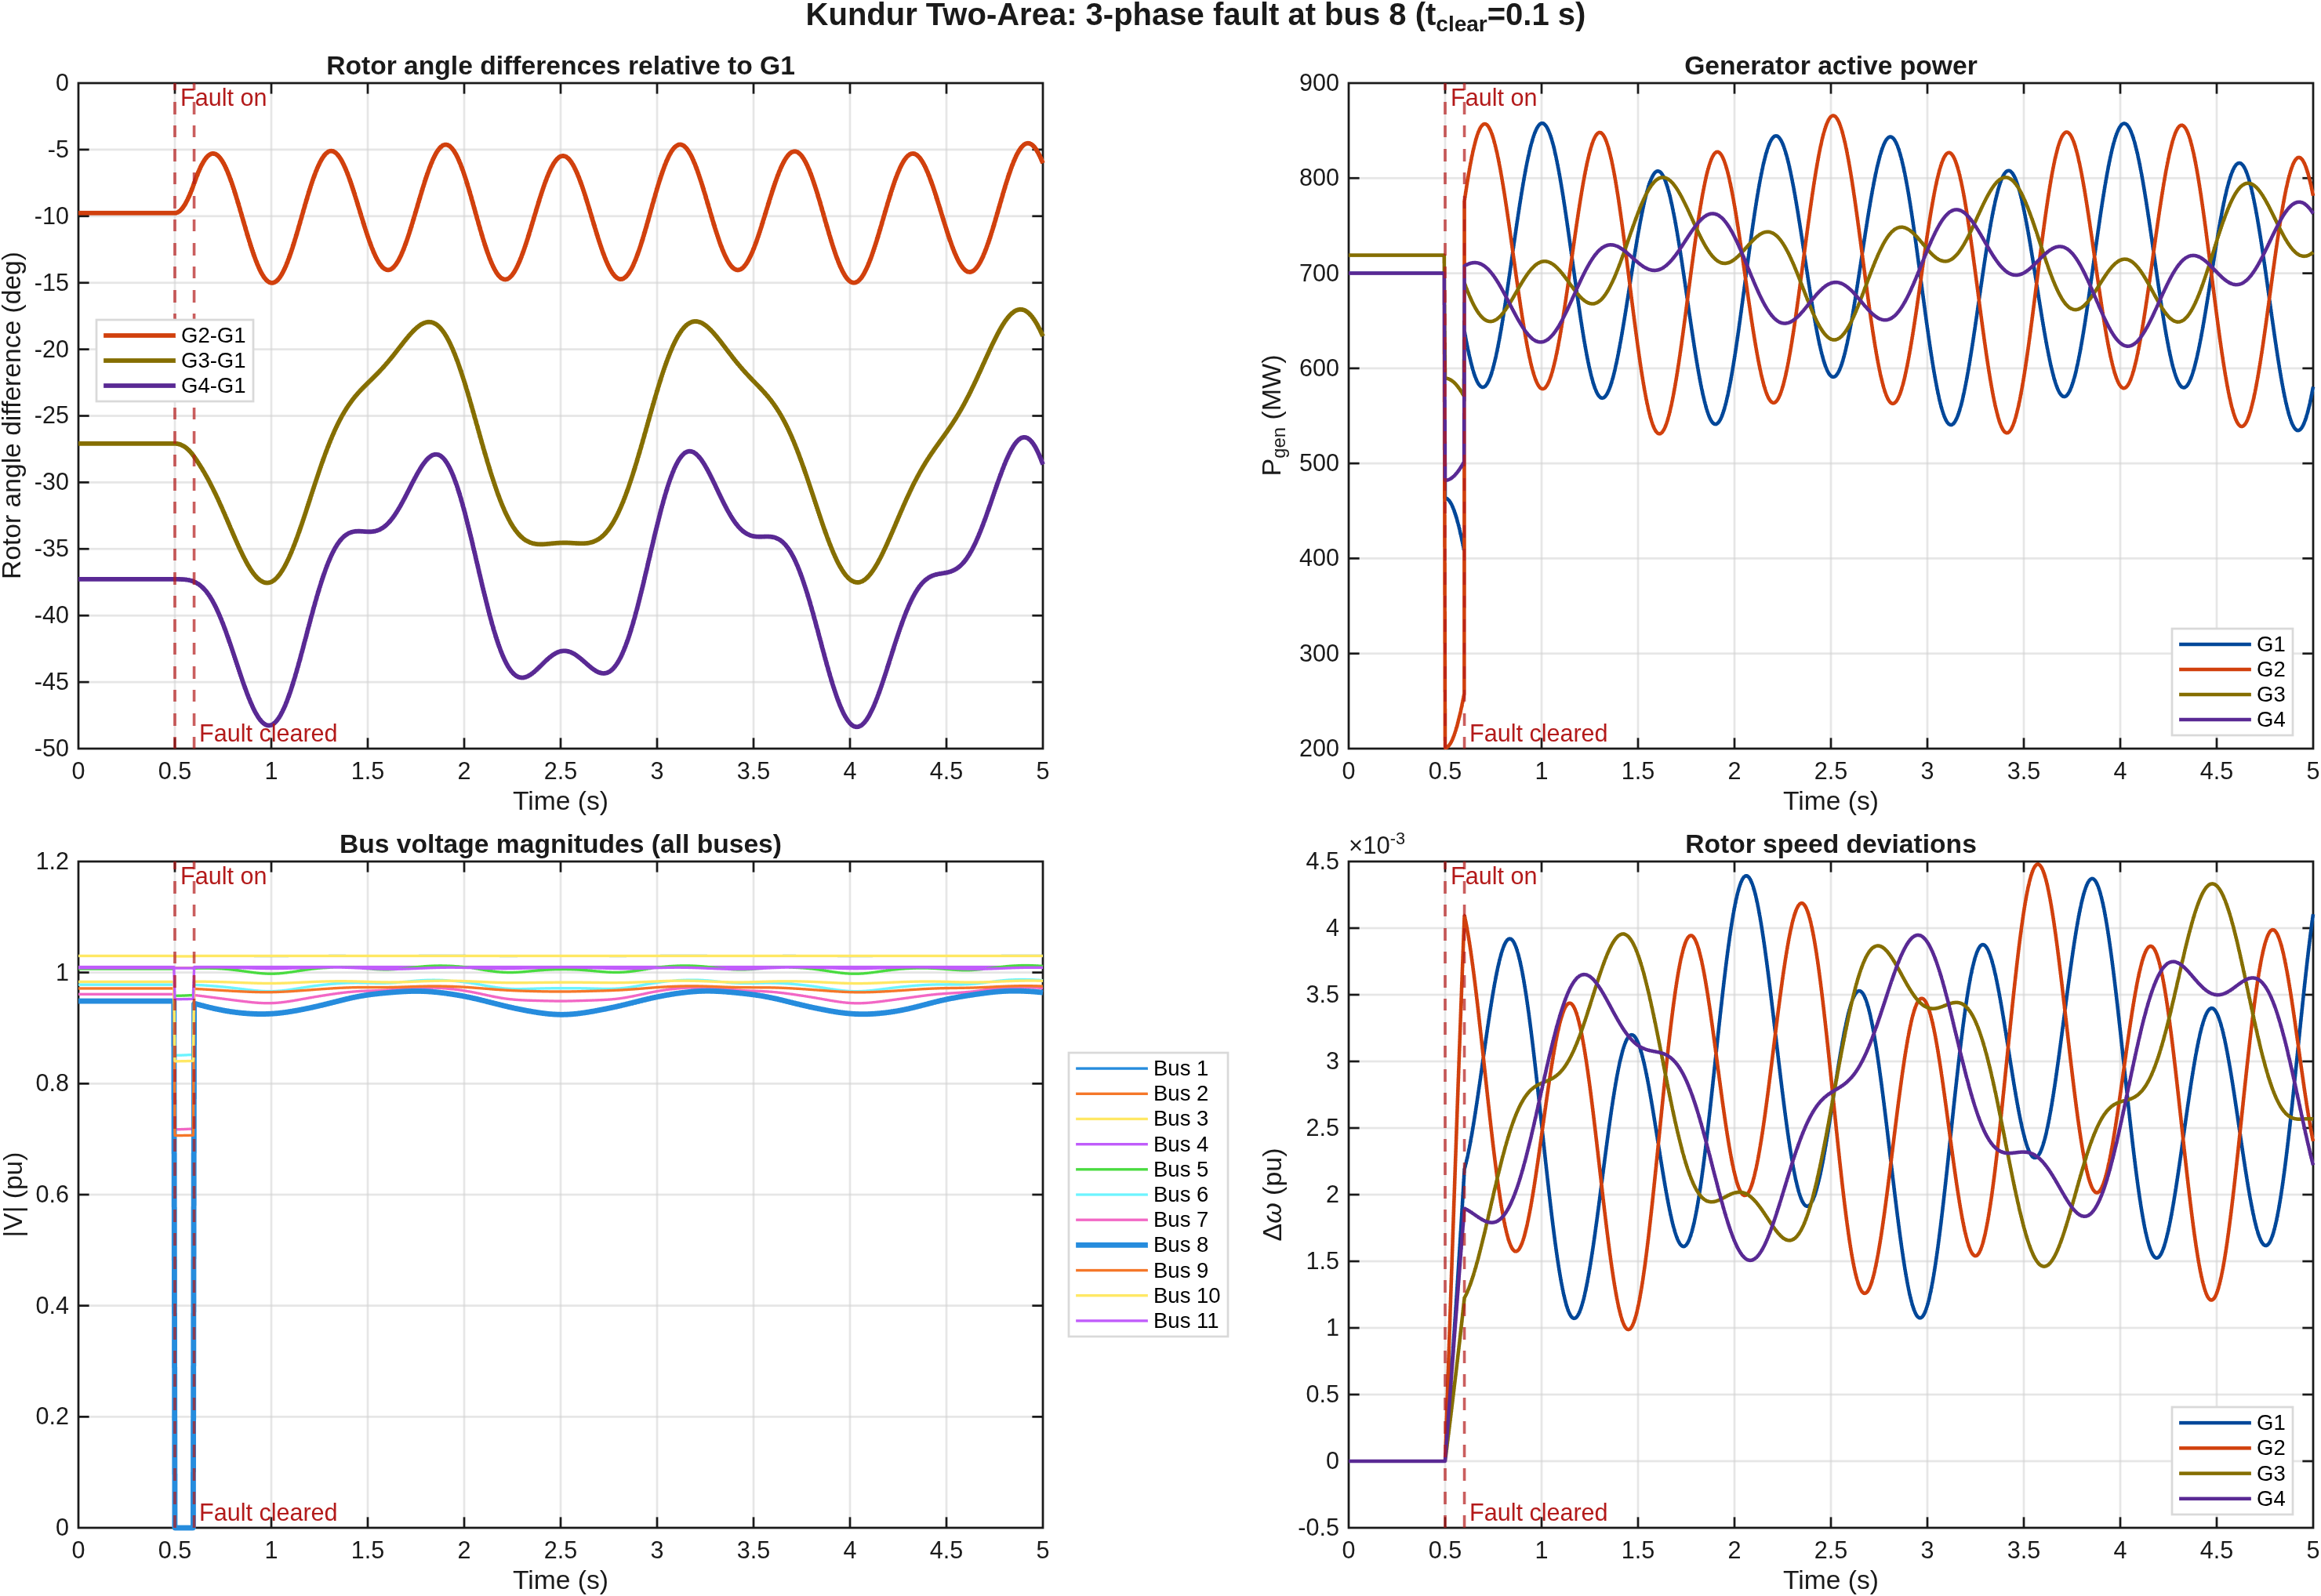
\includegraphics[width=\textwidth]{figures/kundur_ex126/fault_simulation.png}
\caption{Time-domain response to a 3-phase fault at bus~8 ($t_{clear}=0.1$~s).
Top-left: rotor-angle differences relative to G1. Top-right: generator
active power. Bottom-left: bus voltage magnitudes (bus~8 collapses to zero
during the fault). Bottom-right: rotor speed deviations.}
\label{fig:fault}
\end{figure}

\section{Stability Figures}
\label{sec:figs}

Figure~\ref{fig:shapes} shows the rotor-speed mode shapes of the three
rotor-angle modes: the interarea mode has all four machines participating with
opposite signs across the two areas, while the two local modes are confined to
one area. Figure~\ref{fig:eigkd} gives the root locus of the classical SMIB
model as the damping coefficient $K_D$ is swept from $-10$ to $+20$; the
transition from instability ($K_D<0$) to a well-damped swing mode ($K_D>0$) is
clear. Figure~\ref{fig:time} shows a representative time-domain response of
the classical SMIB model that confirms the eigenvalue prediction.

\begin{figure}[H]
\centering
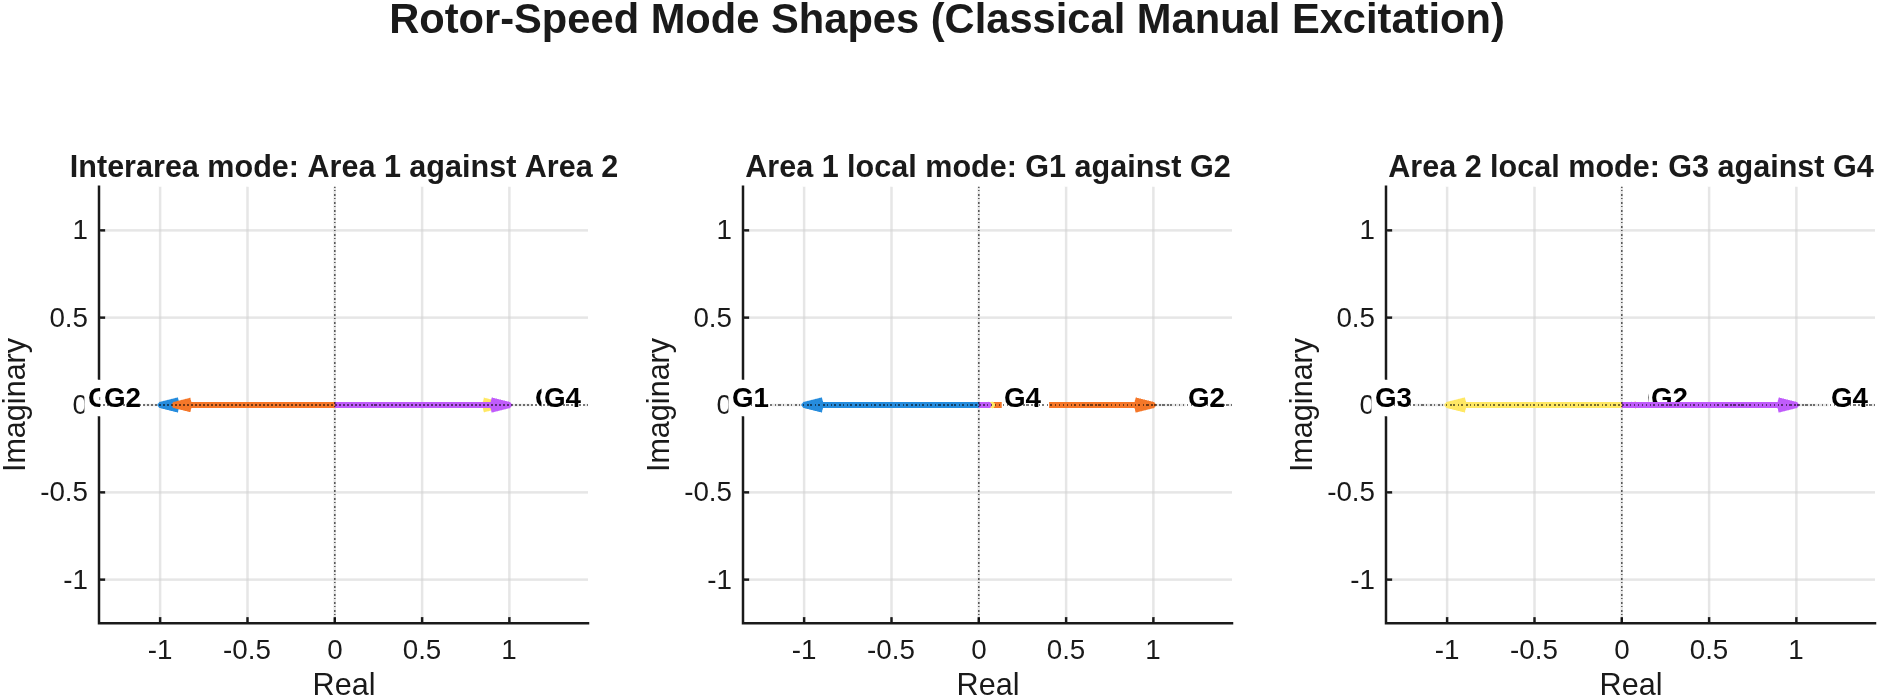
\includegraphics[width=0.95\textwidth]{figures/kundur_ex126/mode_shapes.png}
\caption{Rotor-speed mode shapes for the interarea and local rotor-angle modes
under manual excitation.}
\label{fig:shapes}
\end{figure}

\begin{figure}[H]
\centering
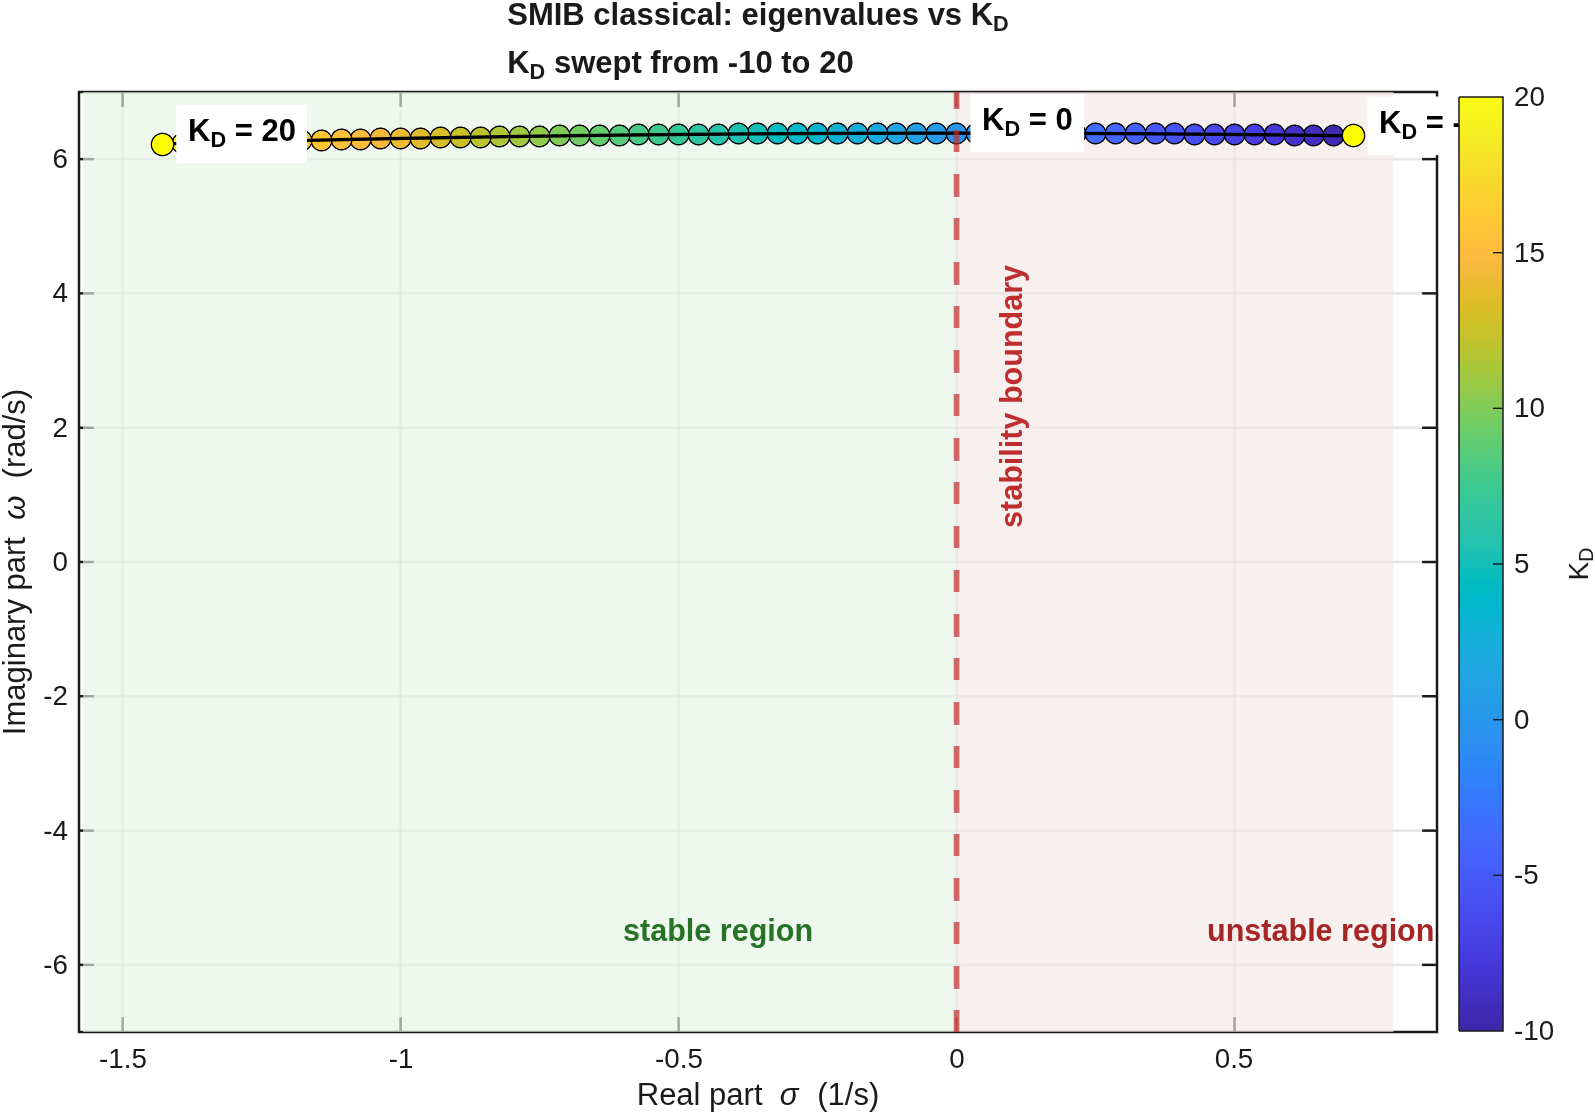
\includegraphics[width=0.95\textwidth]{figures/kundur_ex126/eigenvalues_vs_kd.png}
\caption{Eigenvalue locus of the classical SMIB model as the damping
 coefficient $K_D$ is swept from $-10$ to $+20$. Positive $K_D$ moves the swing
 mode into the stable left-half plane; negative $K_D$ makes it unstable.}
\label{fig:eigkd}
\end{figure}

\begin{figure}[H]
\centering
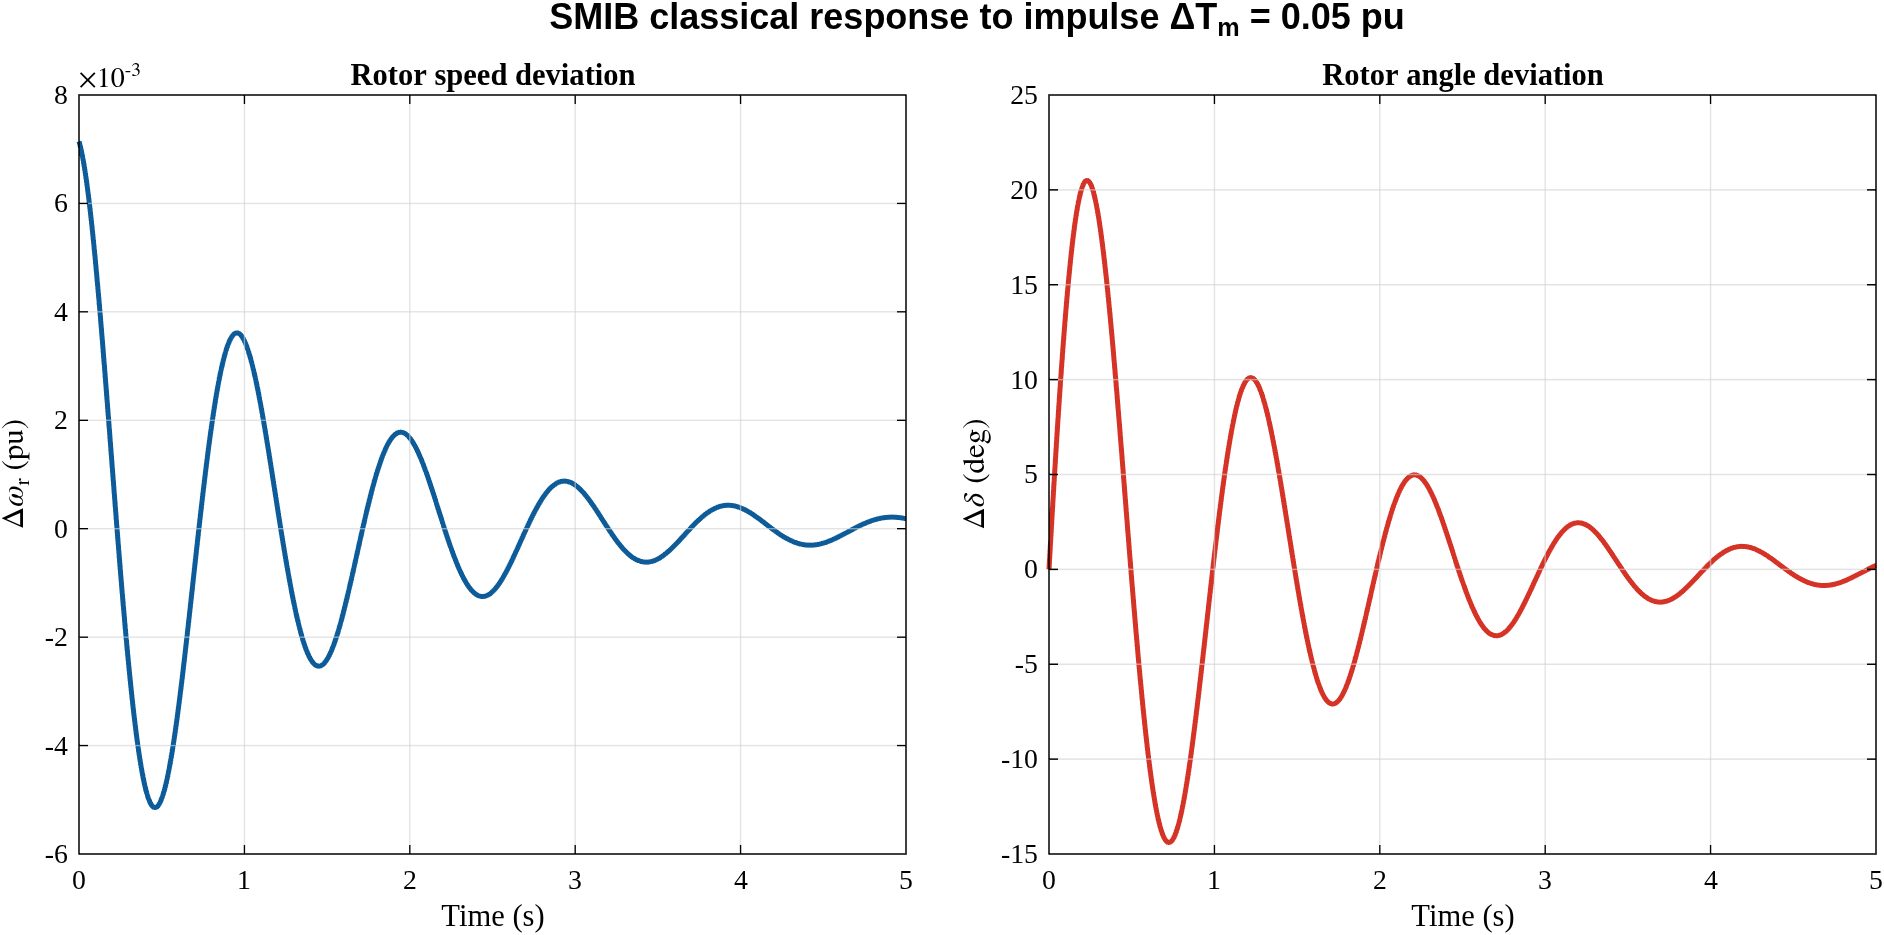
\includegraphics[width=0.95\textwidth]{figures/kundur_ex126/smib_style_time_response.png}
\caption{Representative time-domain response confirming the eigenvalue
prediction of the classical model (damped oscillation at the swing frequency).}
\label{fig:time}
\end{figure}

\section{Conclusion}
\label{sec:concl}

The in-house Newton--Raphson power-flow solver converges for the Kundur
Example~12.6 system in $6$ iterations, yielding a minimum bus voltage of
$0.949$~pu and $85.1$~MW of active losses. Under manual excitation the
small-signal benchmark reproduces Kundur Table~E12.3: the interarea mode at
$0.545$~Hz has a damping ratio of only $0.032$, while the two local modes near
$1.09$--$1.12$~Hz have damping ratios of about $0.072$.
leaving a clean classical/manual-excitation comparison against the textbook.

\end{document}
